\def \Subject {گام دوم: تحقیق بیشتر راجع به موضوع تایید شده}
% \setcounter{chapter}{\Session}
\section{\Subject}
در گام بعد، پس از اینکه موضوع انتخابی توسط دستیاران آموزشی و استاد تایید شد، شروع به تحقیق بیشتر کردم.
با جستجو کردن بیشتر و گشتن داخل فضای اینترنت به جزییات بیشتری در مورد موضوع رسیدم.
در واقع
در این مرحله، موضوع را به صورت کلی‌تر و با جزییات بیشتری مورد بررسی قرار دادم.
ابتدا در این مورد جستجو کردم که 
Zigbee
چیست.
سپس جواب این سوال که چرا 
Zigbee 
بوجود آمده است را پیدا کردم.
در ادامه به بررسی کاربرد های آن پرداختم.
پس از آن به جستجو در مورد انواع دستگاه های آن پرداختم.
بعد از آن معماری شبکه 
Zigbee
را بررسی کردم.
لایه های آن و ویژگی های آن را کنکاش کردم.
در ادامه به بررسی مزایا و معایب آن در مقایسه با دیگر پروتوکل های بیسیم پرداختم.

\begin{figure}[H]
    \centering
    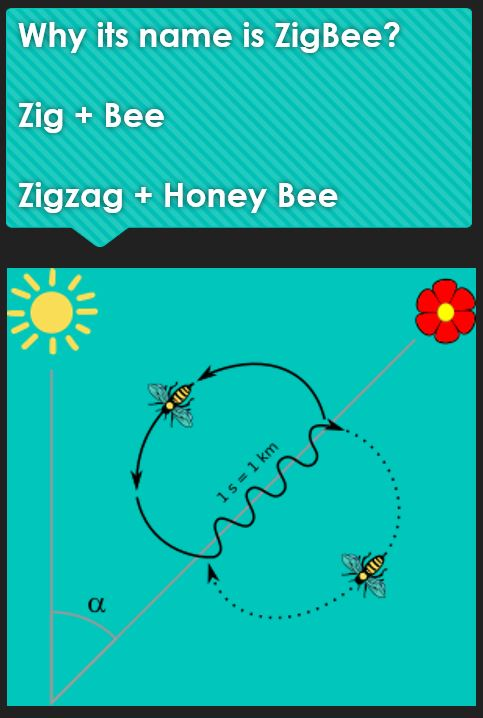
\includegraphics[width=0.65\linewidth]{images/name.JPG}
    \caption{ دلیل نامگذاری Zigbee }
    \label{fig:h}
\end{figure}